\documentclass{beamer}
\usepackage{listings}
\lstset{
%language=C,
frame=single, 
breaklines=true,
columns=fullflexible
}
\usepackage{subcaption}
\usepackage{url}
\usepackage{tikz}
\usepackage{tkz-euclide} % loads  TikZ and tkz-base
%\usetkzobj{all}
\usetikzlibrary{calc,math}
\usepackage{float}
\newcommand\norm[1]{\left\lVert#1\right\rVert}
\providecommand{\brak}[1]{\ensuremath{\left(#1\right)}}
\providecommand{\abs}[1]{\vert#1\vert}
\providecommand{\fourier}{\overset{\mathcal{F}}{ \rightleftharpoons}}
\providecommand{\pr}[1]{\ensuremath{\Pr\left(#1\right)}}
\providecommand{\sbrak}[1]{\ensuremath{{}\left[#1\right]}}
\renewcommand{\vec}[1]{\mathbf{#1}}
\usepackage[export]{adjustbox}
\usepackage[utf8]{inputenc}
\usepackage{amsmath}
\usepackage{mhchem}
\usetheme{Boadilla}

\title{The Pollster's Problem}
\author{Anirudh Srinivasan}
\institute{IIT Hyderabad}
\date{July 2, 2021}
\begin{document}


\begin{frame}
\titlepage
\end{frame}
\begin{frame}{Problem Definition}
\begin{block}{The Pollster's Problem}
The Boss asks pollster to calculate the number of people to be randomly picked as a sample of population to estimate the value of the fraction of population that will vote "yes" in a referendum (denoted by 'p')
\end{block}
\end{frame}

\begin{frame}{Pollster's Initial Approach and its Limitations}
\begin{block}{Steps}
\begin{enumerate}
    \item 'n' people are picked randomly, uniformly and independently over the population and their answers are recorded in indicator random variables 
    \begin{align}
    \pr{X_i} =\begin{cases}
     1, &\text{if yes}  \\
     0, &\text{if no} 
                \end{cases}
    \end{align}
    \item Fraction of "yes" in our sample = $M_n$ = $\frac{X_1+X_2+\dots+X_n}{n}$\\This would be a reasonable estimate for p, however, there is no way to find the exact value of p on the basis of finite and random poll. Hence, there is going to be an error in the estimation of p.
    \item Also, there is no way of guaranteeing the estimate of p with a small error and with certainity as the people polled might not be representative of the true population.
\end{enumerate}
\end{block}
\end{frame}

\begin{frame}{Revised Problem Definition}
\begin{block}{The Pollster's Problem}
\begin{itemize}
    \item The Boss asks Pollster to calculate the number of people to be randomly picked as a sample of population to estimate the value of the fraction of population that will vote "yes" in a referendum (denoted by 'p') with minimal probability of low accuracy.
    \item The desired specifications have 2 parameters:
    \begin{enumerate}
        \item Accuracy of 99\% [1\% margin of error] and 
        \item Probability of an error greater than the margin of error is less than 5\% [95\% confident with the accuracy that is going to be achieved]
    \end{enumerate}
\end{itemize}
\end{block}
\begin{block}{Specifications}
\begin{align}
        \pr{\abs{M_n - p} \geq 0.01} \leq 0.05
    \end{align}
\end{block}
\end{frame}
\begin{frame}{Theorem}
\begin{block}{The Chebyshev's Inequality}
\begin{enumerate}
    \item For a random variable X with finite mean $\mu$ and variance $\sigma^2$,
    \begin{equation}
    \pr{\abs{X-\mu} \geq c} \leq \frac{\sigma^2}{c^2}
    \end{equation}
    where c is any positive real number.
    \item Intuitively, this states that X is unlikely to be too far from the mean if the variance is small.
\end{enumerate}
\end{block}    
\end{frame}
\begin{frame}{Solution}
\begin{block}{}
Consider the i.i.d random variables $X_i$s that act as an indicator that answer is "yes" in the poll. These follow Bernoulli's Distribution with:
    \begin{align}
    \pr{X_i = x} =\begin{cases}
     p, &\text{for x = 1}  \\
     1-p, &\text{for x = 0} 
                \end{cases}\\
    \mu = E[X_i] = \sum_{\forall x}^{} \pr{X_i=x} \times x\\
    \mu = p\times1 + (1-p)\times0 = p
    \end{align}
As $X_i$ is bernoulli random variable, $E[X_i] = E[(X_i)^2] = p$ as x=\{0,1\} is the solution set of $x^2 = x$.
\begin{align}
    \sigma^2 &= E[(X_i)^2] - (E[X_i])^2\\
    &= p - p^2 = p(1-p)
\end{align}
\end{block}
\end{frame}

\begin{frame}{Solution}
\begin{block}{}
Let $M_n$ be the sample mean of the i.i.d random variables $X_i$s. 
    \begin{align}
    M_n = \frac{X_1 + X_2 + X_3 + \dots + X_n}{n}
    \end{align}
    \begin{align}
    E[M_n] = \frac{E[X_1 + X_2 + X_3 + \dots + X_n]}{n} = \frac{n\mu}{n} = \mu = p
    \end{align}
    \begin{align}
        var(M_n) = \frac{var(X_1 + X_2 + X_3 + \dots + X_n)}{n^2} = \frac{n\sigma^2}{n^2} = \frac{\sigma^2}{n} = \frac{p(1-p)}{n}
    \end{align}
\end{block}

\end{frame}

\begin{frame}{Solution - Method 1}
\begin{block}{}
    By applying Chebyshev's Inequality for $M_n$, we get:
    \begin{align}
        \pr{\abs{M_n - \mu} \geq \epsilon} \leq \frac{var(M_n)}{\epsilon^2} = \frac{p(1-p)}{n\epsilon^2} \leq \frac{1}{4n\epsilon^2}
    \end{align}
\end{block}

\begin{block}{}
Comparing this with the desired specifications, we get:
\begin{align}
  \epsilon = 0.01 \text{ and } \frac{1}{4n\epsilon^2} = 0.05   
\end{align}
Solving this, we get: 
n = 50000
\end{block}
\end{frame}

\begin{frame}{Theorem}
\begin{block}{The Central Limit Theorem}
 For a i.i.d random variables $X_1,X_2,\dots,X_n$ with finite mean $\mu$ and variance $\sigma^2$, the random variable given by:
    \begin{align}
    Z_n = \frac{S_n - n\mu}{\sqrt{n}\sigma} \text{ (where: }S_n = X_1+X_2+\dots+X_n)
      \end{align}
follows approximately standard normal distribution for larger n.

\end{block}    
\end{frame}

\begin{frame}{Solution - Method 2}
\begin{block}{}
       We have to rewrite the event $\abs{M_n - p} \geq 0.01$ with an equivalent way involving the standardized normal variable $Z_n$ so that we can use Central Limit Theorem to approximate $\pr{\abs{M_n - p} \geq 0.01}$
\end{block}
\begin{block}{}
\begin{align}
    \abs{M_n - p} \geq 0.01 \implies \left|\frac{S_n}{n} - p\right| \geq 0.01\\ 
    \implies \left|\frac{S_n - np}{n}\right| \geq 0.01 \implies \left|\frac{S_n - np}{\sqrt{n}}\right| \geq 0.01 \sqrt{n} \\
    \implies \left|\frac{S_n - np}{\sqrt{n}\sigma}\right| \geq \frac{0.01 \sqrt{n}}{\sigma} \implies \abs{Z_n} \geq \frac{0.01 \sqrt{n}}{\sigma} \\
    \implies \abs{Z_n} \geq \frac{0.01 \sqrt{n}}{\sqrt{p(1-p)}}
\end{align}
\end{block}

\end{frame}

\begin{frame}{Solution - Method 2}

\begin{block}{}
\begin{align}
    \pr{\abs{M_n - p} \geq 0.01} \approx \pr{\abs{Z} \geq \frac{0.01 \sqrt{n}}{\sqrt{p(1-p)}}} \\
    \pr{\abs{Z} \geq \frac{0.01 \sqrt{n}}{\sqrt{p(1-p)}}} \leq \pr{\abs{Z} \geq 0.02 \sqrt{n}}
\end{align}
\end{block}
\begin{figure}[ht]
    \centering
    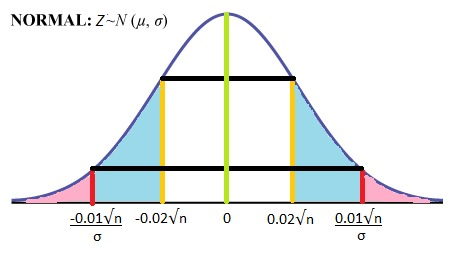
\includegraphics[width=0.5\textwidth]{Normal Distribution.jpeg}
    \caption{Normal Distribution of Z}
    \label{Normal Distribution of Z}
\end{figure}

\end{frame}

\begin{frame}{Solution - Method 2}

\begin{block}{}
\begin{align}
 \pr{\abs{Z} \geq 0.02 \sqrt{n}} = 2\times \pr{Z \geq 0.02 \sqrt{n}}\\
 \pr{Z \geq 0.02 \sqrt{n}} = 1-\phi(0.02\sqrt{n})\\
 \implies \pr{\abs{M_n - p} \geq 0.01} \leq 2 (1-\phi(0.02\sqrt{n}))
\end{align}
\end{block}

\begin{block}{}
Comparing this with the desired specifications, we get:
\begin{align}
  2 (1-\phi(0.02\sqrt{n})) = 0.05\\
  \implies \phi(0.02\sqrt{n}) = 0.975\\
  \implies 0.02\sqrt{n} = 1.96
\end{align}
Solving this, we get: 
n = 9604
\end{block}
\end{frame}

\begin{frame}{Solution - Method 2}
    \begin{figure}[ht]
    \centering
    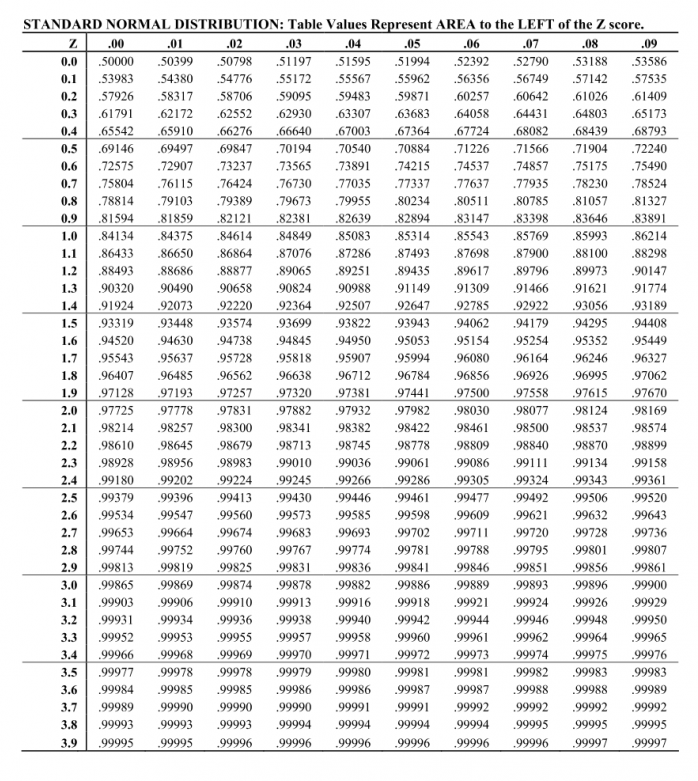
\includegraphics[width=0.5\textwidth]{Z Table - Standard Normal Distribution Table.png}
    \caption{Z Table - Standard Normal Distribution Table}
    \label{Z Table - Standard Normal Distribution Table}
\end{figure}
\end{frame}
\end{document}